\section{Analysis}

In this section, I first motivate the algorithms and techniques that I use for the problem addressed in this project. After this, I present an exploration of the data set used in the project. 

\subsection{Algorithms and Techniques Discussion}
To create software for the classification of students, I want to first reduce the number of features by applying the principal components analysis technique. After this, I will use clustering algorithms to group the students into different groups. In the following, I will briefly explain the general idea of these techniques and motivate their usage in this project. 

\subsubsection{Principal Components Analysis (PCA)}

\paragraph{General Idea.} Principal components analysis is a technique that is frequently used for feature engineering as a preprocessing step for the application of machine learning algorithms. Hereby, the goal is to reduce the number of used features while minimizing the amount of information lost during this reduction process. PCA is performed by creating new features, the so called \emph{principal components} (PCs) that are calculated by a weighted sum of the original features. The weighting factor of each feature hereby depends on the variance of this feature across the data set. Features with a bigger variance are likely to be weighted higher. The underlying idea is that features that are nearly the same across the entire data set (and therefore have a low variance) are unlikely to be useful during a prediction, as they can not be used to distinguish different groups within the data set.

\paragraph{Motivation for the Usage in this project.} There are several reasons why I would like to use PCA before applying clustering algorithms:

\begin{itemize}
	\item \textbf{Reducing the number of features}. When the amount of the available data is limited (which is the case in this project), reducing the number of the features oftentimes improves the performance of machine learning algorithms.
	\item \textbf{Enabling a visualization}. An important advantage of working with 3 or less features is the possibility of a visualization with three or less dimensions that is easily understandable for humans. In this project, we do not have a golden model benchmark (as stated in the analysis section, I would actually expect some deviation from the correctness list). Consequently, it is important to be able to visualize and interpret the results of the clustering. 
	\item \textbf{Finding hidden features}. The PCs found during the PCA oftentimes represent hidden features, that is features which may by rather abstract and not directly measurable, but which at the same time represent characteristics with a high problem relevance (for example the family friendliness of a neighborhood can be a hidden feature when predicting the house prices in the neighborhood). For the problem at hand, these hidden features may be very useful for a usage by the tutors. For example, it is much easier to say whether a student is generally fast when solving problems rather than to specify the exact times he/she needed for the problems.   
\end{itemize}

\subsubsection{Clustering Algorithms}

\paragraph{General Idea.} Clustering describes a group of algorithms from the domain of unsupervised learning. The goal of a clustering algorithm is to identify groups within the provided data objects. To insert problem specific knowledge, clustering algorithms are typically used with a so-called \emph{distance function}. This function takes two data objects and calculates a so-called distance between these. A high distance hereby indicates that the two data objects are not very similar. The goal of clustering algorithms is then to find groups of similar data objects, e.g., of objects with a small distance between them. The exact implementation and the shape of the built clusters depends on the actual algorithm that is being used for clustering.  

\paragraph{Motivation for the Usage in this project.} Unsupervised learning techniques are typically used in situations where it is difficult to label the data. As in our case, the overall problem of the teaching effectiveness is rather complex, I think that it is not enough to consider just one feature of the students, like, e.g., the average correctness, during the student classification. On the other hand, I am not sure how a certain combination of the features present in the data set affects the learning abilities of the students. Clustering, consequently, seems to be a good choice, as it is likely to divide the students into groups based on measurable features. I also hope to gain additional insight into the problem by investigating the clustering results and their correlation with the features of the students.

\subsection{Data Exploration}

Before approaching the actual clustering problem, the data set at hand (or rather the two data sets) have to be explored in order to answer several questions about the characteristics of the data set.

\subsubsection{Split of the KDD data set}

The KDD data set comes in the form of 2 different data sets containing data from different tutoring programs. The first set is called \emph{bridge\_to\_algebra\_2008\_2009}, while the second set is called \emph{algebra\_2008\_2009}. Both sets come within three files: the training file, the test file, and the submission file. The test and the submission files lack most of the data and are provided for the sake of the educational challenge submission. Within this project, I will only be working with the training parts of the two sets. For the sake of brevity, I will refer to the training set of the bridge\_to\_algebra\_2008\_2009 set as \emph{Set A}, while the training set of the algebra\_2008\_2009 will be referred to as \emph{Set B}.

\subsubsection{Checking for missing attributes}

Even a very important feature with great significance for the problem at hand can not be used for the solution of the problem if it is missing in most of the data entries. Consequently, the first step of the data exploration is to examine whether the features in the data set are missing in some of the entries. 

I quantify this by calculating the so-called \emph{feature fraction}. Hereby, a feature that is present in every entry of the entire data set has a feature fraction of $1.0$, while a feature that is only present in every second entry has a feature fraction of $0.5$. The feature fractions of the attributes of Set A and Set B illustrated by the Figs.~\ref{tab_feature_fraction_a} and \ref{tab_feature_fraction_b} are calculated using the script \textbf{\emph{find\_feature\_fraction.py}}.

\begin{figure}[h]
		\centering
		\caption{Feature fractions}
		\label{fig_feature_fractions}
		\subfloat[Set A ($20\,012\,498$ entries)]{\begin{tabular}{cl}
				\toprule
				Attribute name & Feature Fraction \\		
				\midrule
				\colorbox{cyan}{Anon Student Id} & $1.000$ \\
				\colorbox{green}{Error Step Duration (sec)}  & $0.1383$ \\
				\colorbox{red}{Opportunity(SubSkills)} & $0.6198$ \\
				\colorbox{yellow}{Incorrects} & $1.000$ \\
				\colorbox{yellow}{Problem View} & $1.000$ \\
				\colorbox{yellow}{Corrects} & $1.000$ \\
				\colorbox{yellow}{First Transaction Time} & $1.000$ \\
				\colorbox{green}{Step Start Time} & $0.9995$ \\
				\colorbox{yellow}{Hints} & $1.000$ \\
				\colorbox{red}{KC (KTracedSkills)} & $0.5635$ \\
				\colorbox{cyan}{Problem Name} & $1.000$ \\
				\colorbox{cyan}{Problem Hierarchy} & $1.000$ \\
				\colorbox{red}{Opportunity (KTracedSkills)} & $0.5635$ \\
				\colorbox{yellow}{Step End Time} & $1.000$ \\
				\colorbox{yellow}{Correct First Attempt} & $1.000$ \\
				\colorbox{green}{Step Duration (sec)} & $0.9985$ \\
				\colorbox{red}{KC(SubSkills)} & $0.6198$ \\
				\colorbox{green}{Correct Step Duration (sec)} & $0.8602$ \\
				\colorbox{green}{Correct Transaction Time} & $0.9936$ \\
				\colorbox{cyan}{Step Name} & $1.000$\\
				\bottomrule
			\end{tabular}\label{tab_feature_fraction_a}}
		\subfloat[Set B ($8\,918\,054$ entries)]{	\begin{tabular}{cl}
				\toprule
				Attribute name & Feature Fraction \\		
				\midrule
				\colorbox{cyan}{Anon Student Id} & $1.000$ \\
				\colorbox{green}{Error Step Duration (sec)}  & $0.1343$ \\
				\colorbox{red}{Opportunity(SubSkills)} & $0.7223$ \\
				\colorbox{yellow}{Incorrects} & $1.000$ \\
				\colorbox{yellow}{Problem View} & $1.000$ \\
				\colorbox{red}{Opportunity(Rules)} & $0.9639$ \\
				\colorbox{yellow}{Corrects} & $1.000$ \\
				\colorbox{yellow}{First Transaction Time} & $1.000$ \\
				\colorbox{green}{Step Start Time} & $0.9702$ \\
				\colorbox{yellow}{Hints} & $1.000$ \\
				\colorbox{red}{KC (KTracedSkills)} & $0.4956$ \\
				\colorbox{red}{KC(Rules)} & $0.9639$ \\
				\colorbox{cyan}{Problem Name} & $1.000$ \\
				\colorbox{cyan}{Problem Hierarchy} & $1.000$ \\
				\colorbox{red}{Opportunity (KTracedSkills)} & $0.4956$ \\
				\colorbox{yellow}{Step End Time} & $1.000$ \\
				\colorbox{yellow}{Correct First Attempt} & $1.000$ \\
				\colorbox{green}{Step Duration (sec)} & $0.9503$ \\
				\colorbox{red}{KC(SubSkills)} & $0.7223$ \\
				\colorbox{green}{Correct Step Duration (sec)} & $0.8160$ \\
				\colorbox{green}{Correct Transaction Time} & $0.9733$ \\
				\colorbox{cyan}{Step Name} & $1.000$\\
				\bottomrule
			\end{tabular}\label{tab_feature_fraction_b}}		
\end{figure}

\paragraph{Discussion of the Feature Fractions:}

Having calculated the feature fractions, following observations can be made about the attributes in the two data sets:

\begin{itemize}
	\item With more than 20 million entries, the data set A contains more than two times more entries than data set B with about 8 million entries.
	\item The “organizational features” marked \colorbox{cyan}{cyan} describing the name of the student, the name and the hierarchy of the problem, and the name of the step are present for every single entry of both data sets.
	\item The problem solving features marked \colorbox{yellow}{yellow}, namely the problem view, the corrects and incorrects, the number of hints, and the times for the first transaction, the correct first attempt and the step end times are given for every single entry of both data sets.
	\item The KC related features are marked \colorbox{red}{red}. Here, several important things have to be noted:
	\begin{itemize}
		\item The KC features found in the sets are based on different KC models.
		\item Hereby, the set B contains three (SubSkills, KTracedSkills, Rules), and the set A contains two (SubSkills, KTracedSkills) different KC models.
		\item Only a fraction of the steps are mapped to the components of each of the KC models. The Rules model in the set B is the one which is present for the biggest part of the entries.
	\end{itemize}
	\item The time features that are not present for every entry in the data set are marked \colorbox{green}{green}. While they are not present in every single data set, they all can be found in nearly or more than 94\% of the data (the feature fractions of “correct step duration” and the “error step duration” features hereby have to be added, as these features are mutually exclusive).
\end{itemize}

\paragraph{Insights from the feature fraction analysis:}

Based on the results of the feature fraction analysis, I would like to use a subset of the set B as the data set for the remainder of the project. This decision is motivated by multiple circumstances:

\begin{itemize}
	\item The data set B is small enough so that I can process it on my computer without dividing it up into chunks. This also means that I do not have any restrictions for the machine learning algorithms I will be using, as I do not have to rely on their ability to train with subsets of the data set.
	\item Using data set B enables the consideration of the “Rules” model without worrying about the entries where the problem is not mapped on the KC components (the Rules - mapping is present for over 96\% of the data).
	\item Within the chosen set all the features are present for a very big fraction of the entries so that removing entries with missing information does not come at the cost of high information loss.	
\end{itemize}

For the remainder of this project, I would like to use the data set that I will refer to as the \emph{filtered set}. The filtered set is created from the set B by removing all entries that have missing features for the KC class “Rules” or one of the time related features marked green in the above description of the feature fraction. The creation of this set is done by the script \textbf{\emph{filter\_set\_B.py}}. The feature fraction of the resulting set is illustrated in Tab.\ref{tab_ff_filtered_set}.

\begin{table}[h]
	\centering
	\caption{Feature fractions of the filtered set ($8\,035\,374$ entries)\label{tab_ff_filtered_set}. In this set, all attributes are present for all entries. In this set, we keep $90.10\%$ of the data of Set B, so that the information loss is relatively small.}
	\begin{tabular}{cl}
		\toprule
		Attribute name & Feature Fraction \\		
		\midrule
		Opportunity(Rules) &1.0\\ 
		Anon Student Id & 1.0\\ 
		Incorrects & 1.0 \\
		Corrects & 1.0\\ 
		Problem View & 1.0\\ 
		Correct Transaction Time & 1.0\\ 
		Correct First Attempt & 1.0 \\
		Step Duration (sec) & 1.0\\ 
		Correct Step Duration (sec) & 0.87919193307\\ 
		Error Step Duration (sec) & 0.12080806693 \\
		Problem Name & 1.0\\ 
		KC(Rules) & 1.0 \\
		Step Start Time & 1.0\\  
		First Transaction Time & 1.0\\ 
		Problem Hierarchy & 1.0 \\
		Hints & 1.0\\ 
		Step End Time & 1.0\\ 
		Step Name & 1.0\\
		\bottomrule
	\end{tabular}
\end{table}

 \subsubsection{Checking the number of problem steps processed by each student}
 
 Before starting to cluster the students, I examine whether each student in the data set has processed the same amount of problem steps. This is important to assure that a certain group of students does not have a disproportionately big influence on the result of the clustering. At the same time, this is the first step of a transformation of the filtered set, which is focused on the problem steps, into a data set with a focus on the students.
 
During the first step I create a set where each student is annotated with the number of problem steps which he/she solved. This is done by the script called \textbf{\emph{get\_problem\_step\_number.py}}. The results can be found in the file \textbf{\emph{student\_step\_ratio.txt}}. The number of problem steps solved by each students can be described by the values illustrated in Tab.~\ref{tab_number_problem_steps}.

\begin{table}[b]
	\centering
	\caption{Values describing the distribution of the number of problem steps solved by each student. As can be seen, this number is distributed very unequally.\label{tab_number_problem_steps}}
	\begin{tabular}{cl}
		\toprule
		Characteristic & Value \\		
		\midrule
		Overall number of students & $3\,269$ \\
		Maximum number of solved problem steps & $16\,173$ \\
		Minimum number of solved problem steps & $1$ \\
		Average number of solved problem steps & $2\,458.0526$\\
		Standard deviation & $2\,655.444$ \\
		\bottomrule
	\end{tabular}
\end{table}


Investigating the number of problem steps solved by each student shows that this number varies greatly for different students. To prevent the situation where students who have processed a bigger number of problem steps gain an disproportionate influence on the clustering, some kind of normalization has to be performed.

\subsubsection{Normalization of the data set}
Normalizing the filtered set serves two purposes. On the one hand, it addresses the problem that different students have processed different amounts of problem steps. On the other hand, the normalization produces a set where each entry corresponds to a student, as opposed to the filtered set, where each entry corresponds to a problem step. 

The filtered set is normalized using the script \textbf{\emph{make\_student\_data\_set.py}}. The hereby created set is referred to as the \emph{averaged set} and describes each student using the averaged values for the numerical features Incorrects, Problem View, Correct First Attempt, Step Duration (sec), Error Step Duration (sec), Correct Step Duration (sec) and Hints.

\paragraph{Note: } The normalization that I am using can only be applied to numerical values. Consequently, the KC related features, which are represented as one-hot encoded booleans, can not be considered with this approach. While omitting these features comes with a certain information loss, it is \textbf{a)} necessary for the normalization \textbf{b)} probably better to omit these features for the sake of the overall problem, as the KC features offer a very specific description of the mathematical problems they describe and would probably hardly be usable for a tutor. On the other hand, the features that remain in the averaged set are all focused on the correctness of the solution and the time needed for the problem. These features are easily observable for the tutor, regardless of the subject he/she is teaching.

\subsubsection{Correlation Check}
Having determined the features that I want to use for the clustering, I have performed a correlation check to see whether some of the features have strong dependencies to each other. For this, I used the script \textbf{\emph{preprocess\_script.py}}. The results of the correlation analysis are depicted in Fig.

  \begin{figure}
  	\centering
  	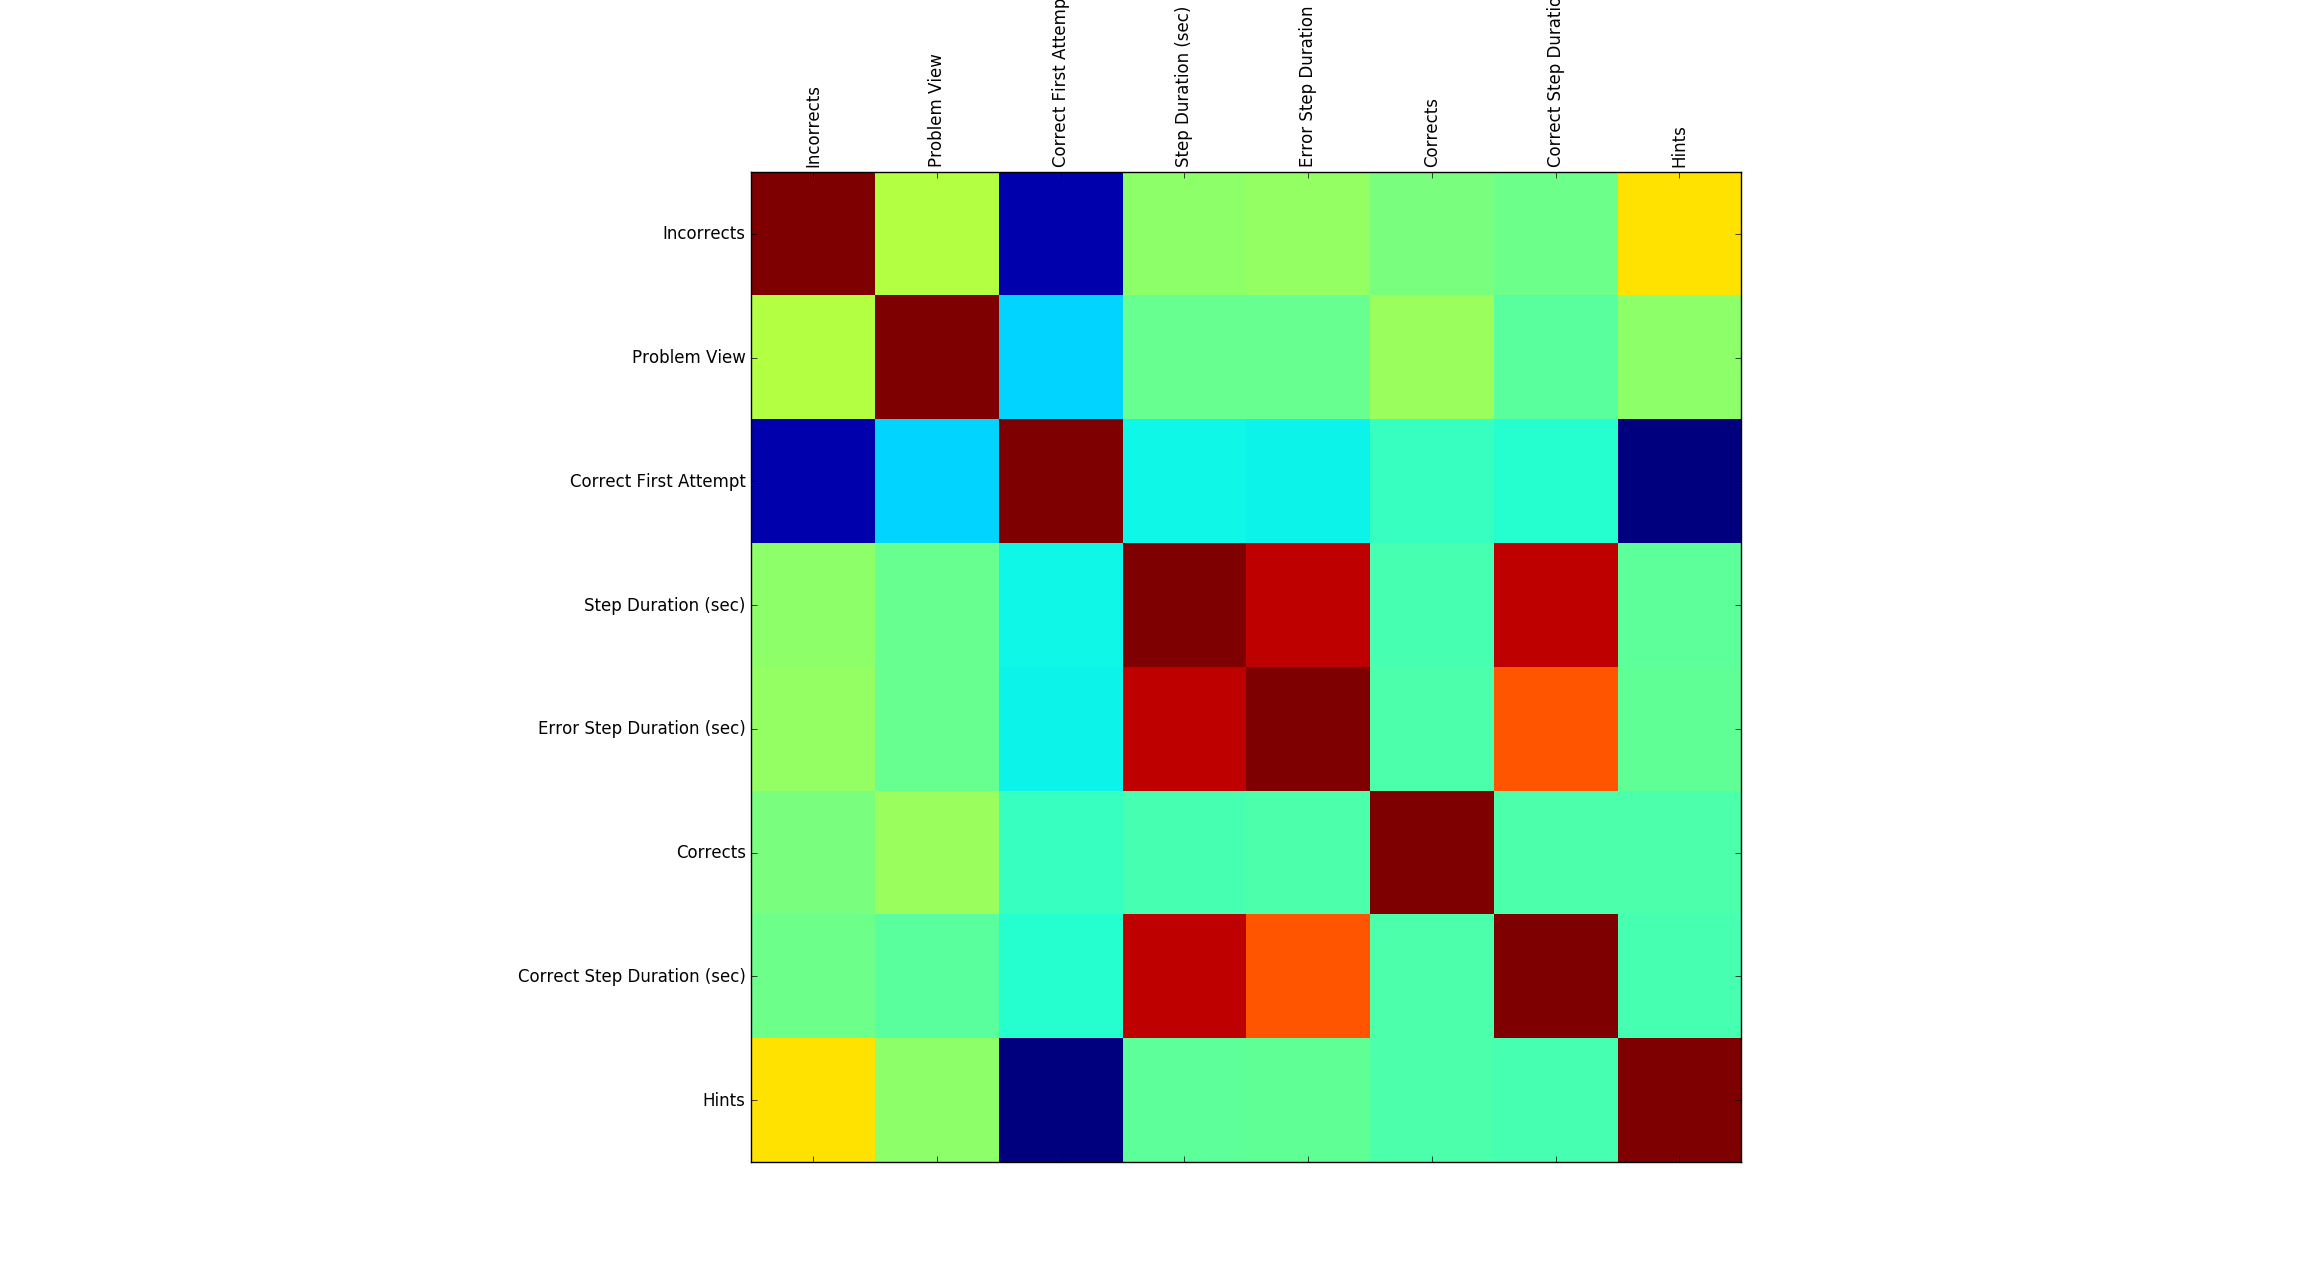
\includegraphics[width=\textwidth]{./img/feature_correlation.png}
  	\caption{Correlation map of the features used in the averaged set.\label{fig_correlations}}
  \end{figure} 
  
 \paragraph{Correlation Discussion:}
 
  The provided image contains a heat map of the correlations between the different values. Cells with a 'warm' color signify a high positive correlation, while 'cold' colors signify negative correlation. Of course, the diagonal of the matrix has the strongest red color. Beside that, there are mainly two facts that can be seen here:
  
  \begin{enumerate}
  	\item Correlation between the Incorrects, the Hints and the Correct First Attempt. Unsurprisingly, these three features correlate with each other. A problem step that is solved correctly on the first attempt does not contribute to the number of incorrects and requires no hints. Consequently, the feature “correct first attempt” has a strong negative correlation with the incorrects and the hints. On the other hand, hints are more likely to be given if the first attempts for a problem solution are incorrect. Consequently, there is a positive correlation between the hints and the number of incorrects.
  	\item Correlation between the step duration, the correct step duration and the error step duration. Unsurprisingly, the step duration strongly correlates with the durations for both the correct and the incorrect steps. There is also a correlation between the time that students need for a correct and an incorrect step.
  \end{enumerate}
  
While there are some correlations in the data set, I do not think that this justifies dropping features. In both correlation situations, there are situations where dropping one of the correlating features would lead to an information loss.


